\documentclass[12pt]{article}
\usepackage{graphicx}
\usepackage{float}
  
%
% Title[Enter title of the experiment here]
\title{EE230: Experiment No.9\\
Instrumentation Amplifier on load cell sensor}

% Author[Enter details of author here]
\author{Aksh Garg, 20D070008}

% begin the document.
\begin{document}

% make a title page.[this creates title page]
\maketitle
 

\section{Overview of the experiment} %[This segment creates Section as seen in document]

\subsection{Aim of the experiment}%[This segment creates sebsections under the same section]

In this experiment, we wish to implement instrumentation amplifier to amplify output from a load cell sensor. In part 1, we will build instrumentation amplifier using TL084 IC. In part 2, we will be using instrumentation amplifier which is available on a PCB on the front panel of a weighing scale(This part is optional). In part 3, we will implement instrumentation amplifier using INA128 IC. This experiment mainly aims at understanding basic three OPAMP instrumentation amplifier and its counterpart in packaged form and comparing the performances of both the configurations.

\subsection{Methods}
First of all, the instrumental ammplifier is made of the required gain using TL084 OPAMP. This circuit is tested using the sine wave generator and the DSO to verify that the circuit is working properly, before connecting it to the weight load machine. After verifying, it is connected to weight load machine according to the instructions given in lab instruction pdf, and the experiment is performed, and the reading is taken. Then, we repeat this part by changing R1 to get double sensitivity.\\
After that, to do Part C, we used IN128 IC. This IC is connected to the weight load machine, and all the required connections are made according to the given instructions, and the experiment is performed, and the reading is taken. Then, we repeat this part by changing Rg to get double sensitivity.\\


\section{Design}%[To add multiple sections, keep appending blocks like this]

\subsection{Load Cell}
\begin{figure}[H]
\begin{center}
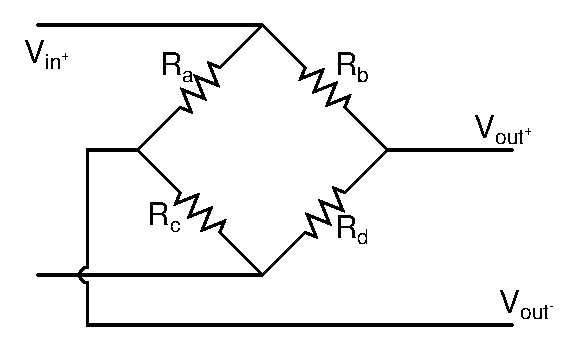
\includegraphics[scale = 0.8]{Lab9-b.eps}
\end{center}
\end{figure}
A load cell is based on an electrical circuit called Wheatstone bridge. It consists of 4 strain gauges connected on a cantilever beam that undergo change in resistance when deformed (i.e. when the object they are connected to experiences strain).\\
This arrangement allows to measure very small changes in the resistance R, which occurs in the strain gauges placed in the arms of the bridge: $R_a$, $R_b$, $R_c$ and $R_d$.\\
When the load cell has no load, the four gauges are at rest and have the same ohmic value, the nominal value of the strain gauge $R_g$:
\begin{equation}
   R_a = R_b = R_c = R_d = R_g 
 \end{equation}
When the load cell experiences deformation due to externally applied force, the resistance of each strain gauge changes by a very small amount $\Delta $R: (when the force is not large enough to make the response of the sensors non-linear).\\
\begin{equation}
  R_a=R_g+\Delta R ; R_b=R_g -\Delta R ; R_c=R_g -\Delta R ; R_d=R_g+\Delta R
 \end{equation}
Strain gauges placed on opposite faces of the cantilever present opposite polarity of change in resistance.\\

\subsection{Instrumental Amplifier}
\begin{figure}[H]
\begin{center}
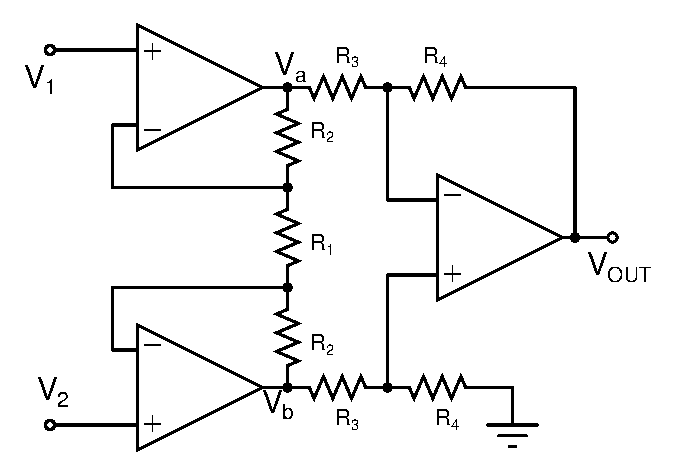
\includegraphics[scale = 0.8]{Lab9-a.eps}
\end{center}
\end{figure}
An instrumentation amplifier is a type of differential amplifier that has been outfitted with input buffer amplifiers. These input buffers eliminate the need for input impedance matching and thus make the amplifier particularly suitable for use in measurement and test equipment. Additional characteristics include very low DC offset, low drift, low noise, very high open-loop gain, very high common-mode rejection ratio, and very high input impedance. Instrumentation amplifiers are used to achieve high accuracy and stability. \\
Here, we define the input voltage signals small signal AC differential input $V_1$ and $V_2$, as the input of first stage OPAMPs of the instrumentation amplifier. We assume input resistance of OPAMPs to be infinite. Now applying KCL at inverting input of first stage OPAMPs. We get,
\begin{equation}
   V_a = V_1(1 + R_2/R_1) + V_2(R_2/R_1)
 \end{equation}
And,
\begin{equation}
   V_b = -V_1(R_2/R_1) + V_2(1 + R_2/R_1)
 \end{equation}
Using superposition principle of voltages at second stage OPAMP,
\begin{equation}
  V_{out} = R_4/R_3(1 + 2R_2/R_1)(V_2 - V_1)
 \end{equation}
Rearranging this equation, the gain is
\begin{equation}
  A_v = V_{out}/(V_1 - V_2) = (R_4/R_3)(1 + 2R_2/R_1)
 \end{equation}
As we want the gain of 300, we take R1 = 1k$\Omega $, R2 = 6.8k$\Omega $, R3 = 1k$\Omega $, R4 = 22k$\Omega $. This will give gain as 321, we also have resistors availability constrain in labs, so this is approx 300 of gain here.\\
This is used in Part A of this experiment and the OPAMP used is TL084.


\subsection{Part-C}
\begin{figure}[H]
\begin{center}
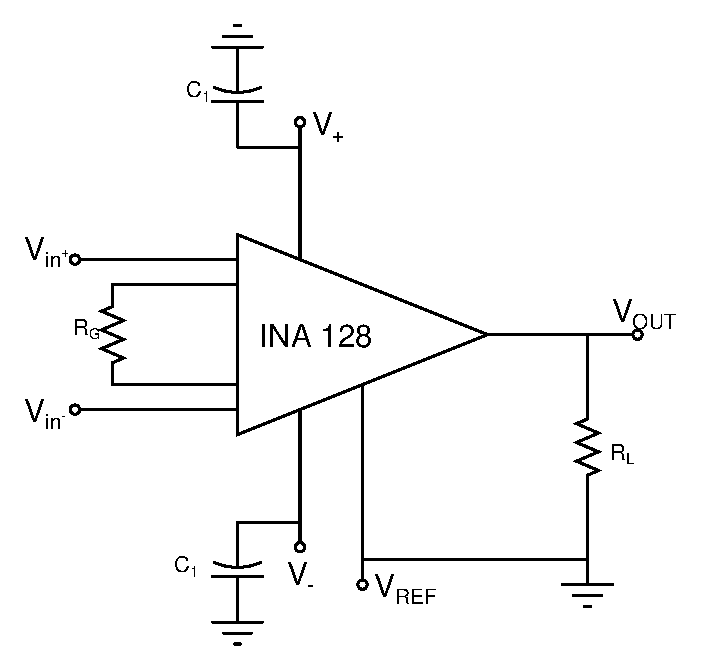
\includegraphics[scale = 0.8]{Lab9-c.eps}
\end{center}
\end{figure}
In this part, we need not to use instrumental amplifier directly, as we had done in Part-A. Here, we use IN128 opamp amplifier, and connect it accordingly with the weight scale machine as given in the lab pdf, and do the experiment.

\section{Simulation results}%[One more section]
\subsection{Code snippet}

\begin{center}
\textbf{Instrumental Amplifier}
\end{center}
.include TL084.txt\\
x1 1 2 3 4 5 TL084\\
x2 6 7 3 4 10 TL084\\
x3 8 9 3 4 11 TL084\\
*amplification of just 30\\
r1 2 7 1k\\
r2x 2 5 1k\\
r2 7 10 1k\\
r3 8 10 1k\\
r3x 9 5 1k\\
r4 9 11 10k\\
r4x 8 0 10k\\
vcc 3 0 12\\
vdd 4 0 -12\\
v1 1 0 sin(0 100m 1k 0 0)\\ 
v2 6 0 sin(0 -100m 1k 0 0) \\
.tran 5u 5m\\
.control\\
run\\
plot v(11) v(1)-v(6)\\
.endc\\
.end\\

\subsection{Simulation results}


\begin{figure}[H]
\begin{center}
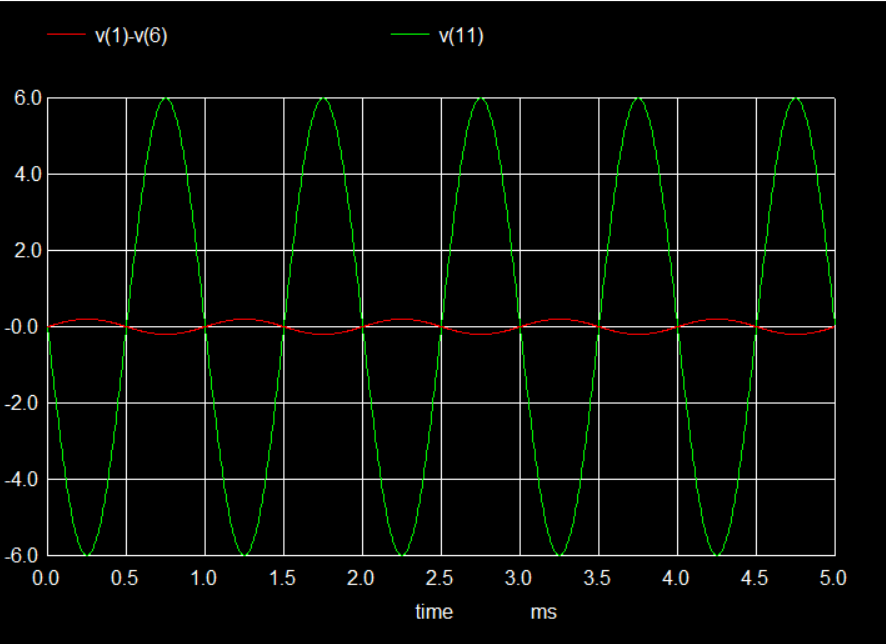
\includegraphics[scale = 0.6]{b.png}
\caption{$V_{OUT}$ vs V1-V2}
\end{center}
\end{figure}


\section{Experimental results}
\subsection{Part-A}
\begin{center}
\textbf{R1 = 1k$\Omega $, R2 = 6.8k$\Omega $, R3 = 1k$\Omega $, R4 = 22k$\Omega $}
\end{center}
\begin{center}
\begin{table}[H]
		% Center the table
		\begin{center}
		
		\begin{tabular}{|c|c|}
			% To create a horizontal line, type \hline
			\hline
			% To end a column type &
			% For a linebreak type \\
			\textbf{Weight(gm)} & \textbf{$V_{OUT}$ (mV)}\\
			\hline
			1 & 179\\
			\hline
			2 & 176.5\\
			\hline
                   3 & 173\\
			\hline
                   5 & 166\\
			\hline
                   7 & 161.5\\
			\hline
                   8 & 159\\
			\hline
50 & 61\\
			\hline
100 & -60\\
			\hline
150 & -180\\
			\hline
            
		\end{tabular}
		\end{center}
\end{table}
\end{center}
\begin{figure}[H]
\begin{center}
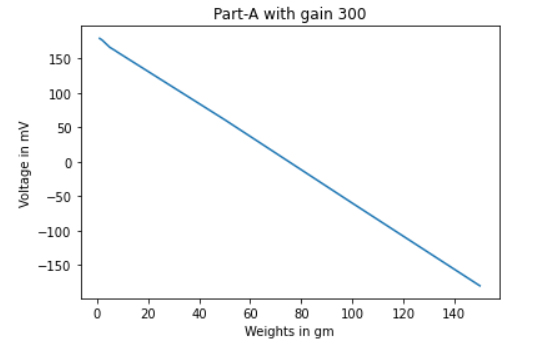
\includegraphics[scale = 1]{ai.PNG}
\end{center}
\end{figure}
Here. the gain of instrumental amplifier is 321.\\
This results in the sensitivity as -2.4mV/gm\\

\begin{center}
\textbf{R1 = 470$\Omega $, R2 = 6.8k$\Omega $, R3 = 1k$\Omega $, R4 = 22k$\Omega $}
\end{center}
\begin{center}
Here, we try to double the sensitivity with the resources available in lab.
\begin{table}[H]
		% Center the table
		\begin{center}
		
		\begin{tabular}{|c|c|}
			% To create a horizontal line, type \hline
			\hline
			% To end a column type &
			% For a linebreak type \\
			\textbf{Weight(gm)} & \textbf{$V_{OUT}$ (mV)}\\
			\hline
			1 & 380\\
			\hline
			2 & 374.5\\
			\hline
                   3 & 369.4\\
			\hline
                   5 & 359\\
			\hline
                   7 & 348\\
			\hline
                   8 & 343\\
			\hline
50 & 125\\
			\hline
100 & -135\\
			\hline
150 & -386\\
			\hline
            
		\end{tabular}
		\end{center}
\end{table}
\end{center}
\begin{figure}[H]
\begin{center}
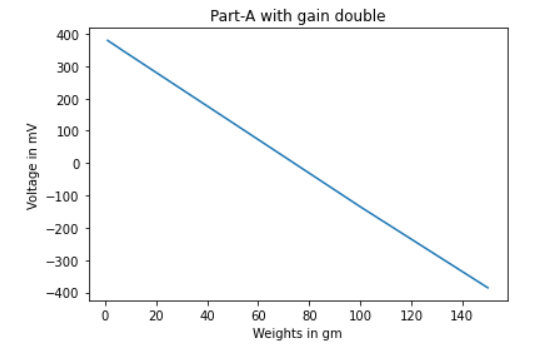
\includegraphics[scale = 1]{aii.PNG}
\end{center}
\end{figure}
Here. the gain of instrumental amplifier is 658.\\
This results in the sensitivity as -5.1mV/gm\\



\subsection{Part-C}
\begin{center}
\textbf{Rg = 220$\Omega $}
\end{center}
\begin{center}
\begin{table}[H]
		% Center the table
		\begin{center}
		
		\begin{tabular}{|c|c|}
			% To create a horizontal line, type \hline
			\hline
			% To end a column type &
			% For a linebreak type \\
			\textbf{Weight(gm)} & \textbf{$V_{OUT}$ (mV)}\\
			\hline
			1 & -190\\
			\hline
			2 & -192\\
			\hline
                   5 & -198\\
			\hline
                   8 & -203\\
			\hline
50 & -274\\
			\hline
100 & -358\\
			\hline
150 & -444\\
			\hline
            
		\end{tabular}
		\end{center}
\end{table}
\end{center}
\begin{figure}[H]
\begin{center}
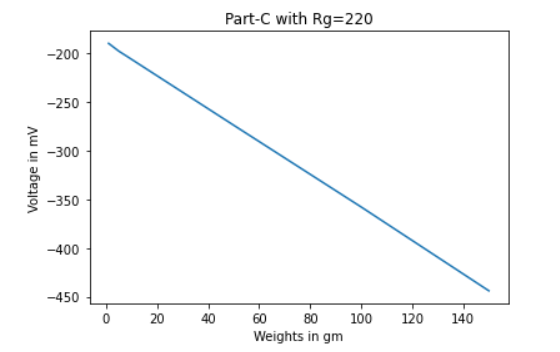
\includegraphics[scale = 1]{ci.PNG}
\end{center}
\end{figure}
This results in the sensitivity as -1.7mV/gm\\

\begin{center}
\textbf{Rg = 100$\Omega $}
\end{center}
\begin{center}
Here, we try to double the sensitivity with the resources available in lab.
\begin{table}[H]
		% Center the table
		\begin{center}
		
		\begin{tabular}{|c|c|}
			% To create a horizontal line, type \hline
			\hline
			% To end a column type &
			% For a linebreak type \\
			\textbf{Weight(gm)} & \textbf{$V_{OUT}$ (mV)}\\
			\hline
			1 & -419\\
			\hline
			2 & -422\\
			\hline
                   5 & -435\\
			\hline
                   8 & -447\\
			\hline
50 & -603\\
			\hline
100 & -787\\
			\hline
150 & -975\\
			\hline
            
		\end{tabular}
		\end{center}
\end{table}
\end{center}
\begin{figure}[H]
\begin{center}
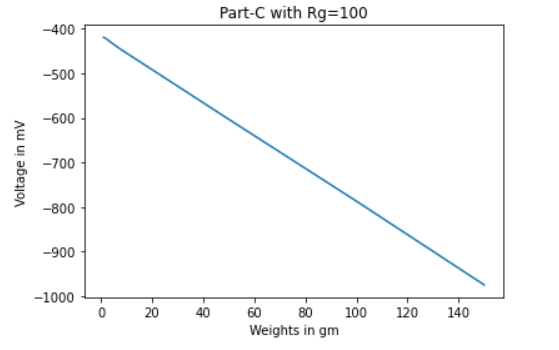
\includegraphics[scale = 1]{cii.PNG}
\end{center}
\end{figure}
This results in the sensitivity as -3.7mV/gm\\





\section{Experiment completion status}
All the parts of this experiment are completed successfully.

  

\end{document}
